\subsection{Descripción del algoritmo implementado.}
\vspace*{0.3cm}

La \textbf{heurística de búsqueda local} consiste en comenzar con una
solución dada, definir el concepto de solución ``vecina'', generar estas
soluciones vecinas y revisar si alguna es mejor a la actual.

De existir, se toma esta como solución actual y se repite el proceso
buscando las vecinas de la nueva solución.

\vspace*{0.3cm}

Para nuestro algoritmo, planteamos las siguientes 2 vecindades:

\begin{itemize}
    \item mover: Una partición es vecina de otra si consiste en mover un único vértice de un conjunto a otro.
    \begin{align*}
        v \in V, u \in U, v \ne u \\
        V \setminus \{v\} = U \setminus \{u\}
    \end{align*}

    \item intercambiar: Una partición es vecina de otra si consiste en intercamiar 2 vértices de distintos conjuntos.
    \begin{align*}
        v \in V, u \in U \\
        V' = V \setminus \{v\} \cup \{u\} \\
        U' = U \setminus \{u\} \cup \{v\}
    \end{align*}
\end{itemize}

Los algoritmos consisten en, partiendo de una solución inicial, probar sobre todas las vecinas, y continuar desde la de menor peso. Cuando no se pueda mejorar más, finaliza la ejecución.

\vspace*{0.5cm}

\textbf{Pseudocódigo con la estrategia mover:}

\vspace*{0.3cm}

\begin{verbatim}
kpmp_mover(particion) {
    pesoMin = peso(particion)
    sePuedeMejorar = true
    mientras sePuedeMejorar {
        por cada vertice en vertices(particion) {
            conjuntoDelVertice = buscarConjunto(particion, vertice)
            pesoSinVertice = peso(particion) - costo(conjuntoDelVertice, vertice)
            por cada conjunto en conjuntos(particion) excepto conjuntoDelVertice {
                peso = pesoSinVertice + costo(conjunto, vertice)
                si peso < pesoMin {
                    pesoMin = peso
                    verticeMin = vertice
                    conjuntoViejo = conjuntoDelVertice
                    conjuntoNuevo = conjunto
                }
            }
        }
        si pesoMin < peso(particion) {
            sacarVertice(conjuntoViejo, verticeMin)
            agregarVertice(conjuntoNuevo, verticeMin)
        } sino {
            sePuedeMejorar = false
        }
    }
}
\end{verbatim}

\newpage

\textbf{Pseudocódigo con la estrategia intercambiar:}

\vspace*{0.3cm}

\begin{verbatim}
kpmp_switch(particion) {
    pesoMin = peso(particion)
    sePuedeMejorar = true
    mientras sePuedeMejorar {
        por cada vertice1 en vertices(particion) {
            conjuntoDelVertice1 = buscarConjunto(particion, vertice)
            por cada vertice2 en vertices(particion) excepto que compartan conjunto {
                conjuntoDelVertice2 = buscarConjunto(particion, vertice)
                peso = peso(particion)
                    - costo(conjuntoDelVertice1, vertice1)
                    - costo(conjuntoDelVertice2, vertice2)
                    + costo(conjuntoDelVertice1, vertice2)
                    + costo(conjuntoDelVertice2, vertice1)
                si peso < pesoMin {
                    pesoMin = peso
                    verticeMin1 = vertice1
                    verticeMin2 = vertice2
                    conjuntoMin1 = conjuntoDelVertice1
                    conjuntoMin2 = conjuntoDelVertice2
                }
            }
        }
        si pesoMin < peso(particion) {
            sacarVertice(conjuntoDelVertice1, verticeMin1)
            agregarVertice(conjuntoDelVertice1, verticeMin2)
            sacarVertice(conjuntoDelVertice2, verticeMin2)
            agregarVertice(conjuntoDelVertice2, verticeMin1)
        } sino {
            sePuedeMejorar = false
        }
    }
}
\end{verbatim}



\newpage
\subsection{Análisis de complejidad del peor caso de una iteración del
            algoritmo de búsqueda local.}
\vspace*{0.3cm}

Sea $G = (V,E)$ y consideremos $n = |V|$ y $m = |E|$.

La función \texttt{buscarConjunto} recorre todos los conjuntos y en cada uno
busca, en tiempo logarítmico, el vértice dado. Esta función realiza sobre cada
conjunto $O(\log(\text{cantidad de vértices del conjunto}))$ comparaciones,
realizadas en $O(1)$. A su vez, la cantidad de elementos de cada conjunto está
acotada por $n$. Luego, la complejidad de esta función es $O(k\log(n))$, siendo
$k$ el parámetro de entrada.

\vspace*{0.3cm}

En cada iteración, el algoritmo de búsqueda local con la estrategia de
\textit{mover} comienza a recorrer cada vértice del grafo, realizando lo siguiente:
\begin{itemize}
  \item Se llama a la función \texttt{buscarConjunto}, la cual pertenece a
  $O(k\log(n))$.

  \item Por cada conjunto de la partición, se calcula el peso obtenido al
  agregarlo al conjunto, llamando a la función \texttt{costo}. Al igual que en
  la función \texttt{agregarAlDeMenosPeso} explicada en el ítem anterior, esto
  pertenece a $O(k + n)$.
\end{itemize}

Luego de recorrer cada vértice, se pueden llegar a realizar 2 llamados a
la función \texttt{costo}, que pertenece a $O(n)$.

Por lo tanto, en cada iteración del algoritmo de busqueda local, la complejidad
es $O(n (k\log(n) + k + n) + n)$, que tomando solo en cuenta los casos donde
$k < n$, se reduce a $O(n (n\log(n) + n + n) + n) = O(n^2 \log(n))$.

\vspace*{0.3cm}

En cada iteración, el algoritmo de búsqueda local con la estrategia de
intercambiar comienza a recorrer cada vértice del grafo, realizando lo siguiente:

\begin{itemize}
  \item Se llama a la función \texttt{buscarConjunto}, la cual pertenece a
  $O(k\log(n))$.

  \item Por cada uno de los otros vértices que no están en el mismo conjunto
  que el vértice actual:

  \begin{itemize}
    \item Se llama de nuevo a la función \texttt{buscarConjunto}.

    \item Se llama 4 veces a la función \texttt{costo}.
  \end{itemize}
\end{itemize}

Finalmente, se pueden llegar a realizar 4 llamados más a la función
\texttt{costo}.

Por lo tanto, en cada iteración del algoritmo de búsqueda local, la complejidad
es $O(n (k\log(n) + n (k\log(n) + k + n)) + k + n)$. Nuevamente, sólo
considerando los casos donde $k \le n$, la complejidad se reduce a
$O(n(n\log(n) + n (n\log(n) + n + n)) + n + n) = O(n (n\log(n) + n^2 \log(n)) + n) = O(n^3 \log(n))$.



\newpage \subsection{Experimentación y gráficos.}
\vspace*{0.3cm}

\vspace*{0.3cm}

\subsubsection{Test 1 - algoritmo goloso, sin aleatorización}

(ver \verb|info.greedy.dat.promedio|) \medskip

En este test, tenemos $n$ nodos, con $n$ inicializado en 100, incrementándose de a 10 hasta alcanzar 1000, $m$ inicializado en 500, incremendtándose de a 50 hasta alcanzar 5000 (vale 5 veces $n$) y $k$ vale $\frac{n}{20}$.

Para cada instancia se toma el \textbf{valor mínimo} mediado en microsegundos luego de \textbf{10 corridas}.

Dada una combinación de $m$, $n$ y $k$, se generaron 5 instancias aleatorias con dicha combinación y se consideró el promedio entre ellas.

\vspace*{0.5cm}

\begin{figure}[h]
  \begin{center}
    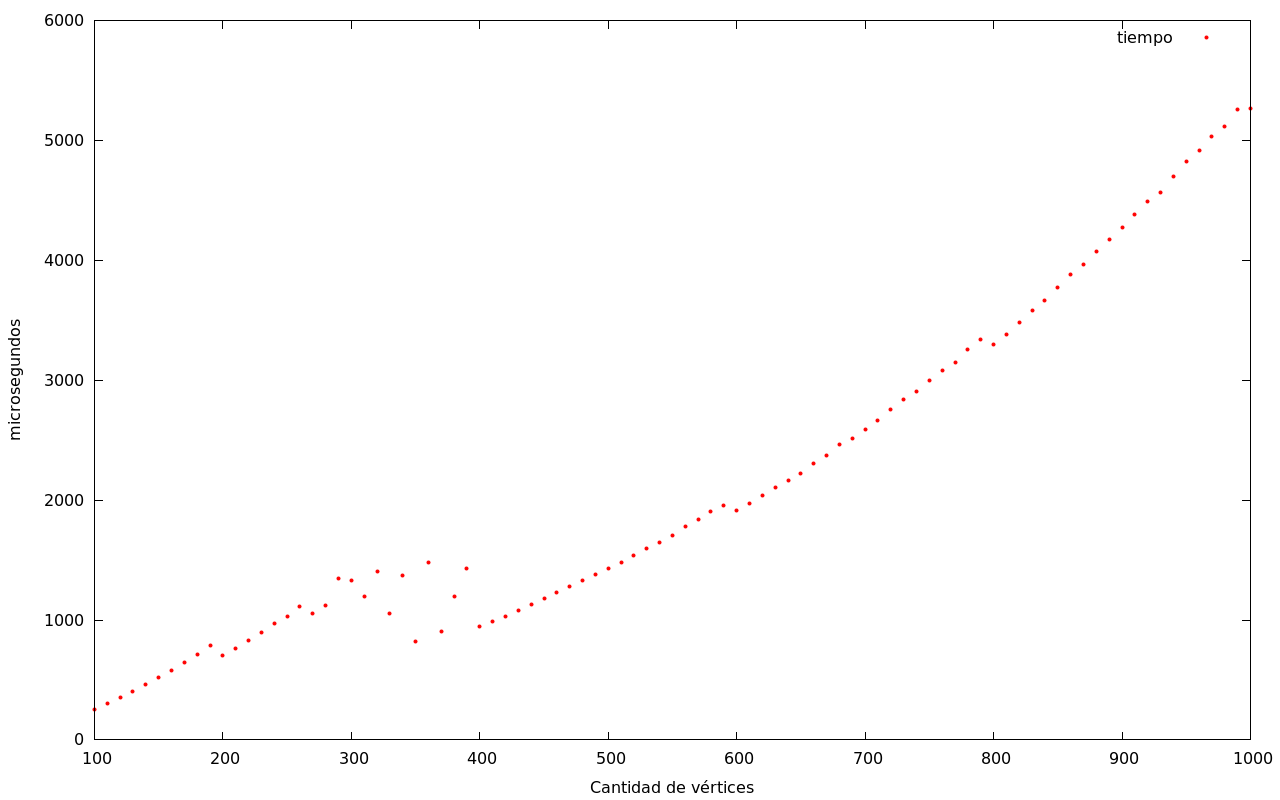
\includegraphics[scale=0.35]{imagenes/grafico-greedy-ac.png}
  \end{center}
\end{figure}

\vspace*{0.5cm}


\newpage
\subsubsection{Test 2 - algoritmo goloso, con aleatorización en las aritas}

(ver \verb|info.2.k.dat|) \medskip

En este test, tenemos $n$ nodos, con $n$ inicializado en 100, incrementándose de a 10 hasta alcanzar 1000, $m$ inicializado en 500, incremendtándose de a 50 hasta alcanzar 5000 (vale 5 veces $n$) y $k$ vale $\frac{n}{20}$.

Para cada instancia se toma el \textbf{valor mínimo} mediado en microsegundos luego de \textbf{10 corridas}.

Dada una combinación de $m$, $n$ y $k$, se generaron 5 instancias aleatorias con dicha combinación y se consideró el promedio entre ellas.

\vspace*{0.5cm}

\begin{figure}[h]
  \begin{center}
    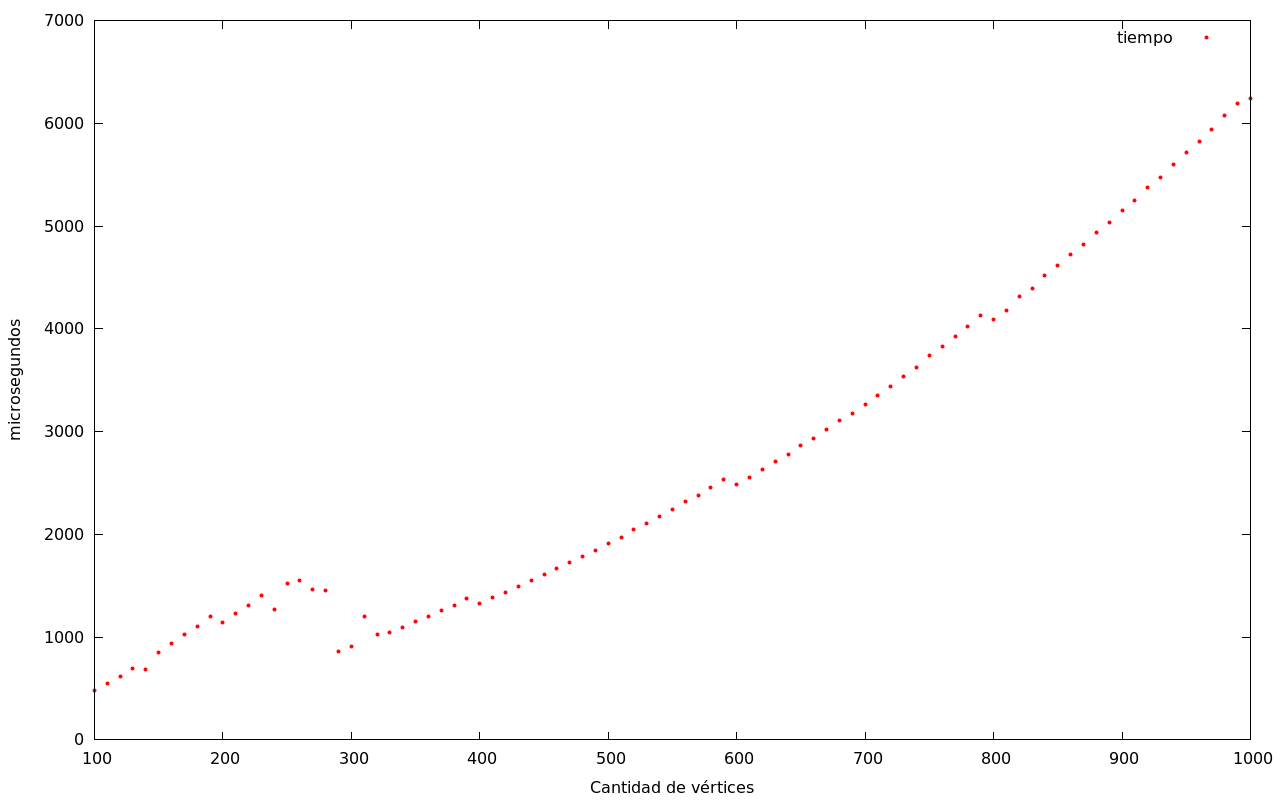
\includegraphics[scale=0.35]{imagenes/grafico-greedy-a.png}
  \end{center}
\end{figure}

\vspace{0.5cm}


\newpage
\subsubsection{Test 3 - algoritmo goloso, con aleatorización en conjuntos}

(ver \verb|info.2.k.dat|) \medskip

En este test, tenemos $n$ nodos, con $n$ inicializado en 100, incrementándose de a 10 hasta alcanzar 1000, $m$ inicializado en 500, incremendtándose de a 50 hasta alcanzar 5000 (vale 5 veces $n$) y $k$ vale $\frac{n}{20}$.

Para cada instancia se toma el \textbf{valor mínimo} mediado en microsegundos luego de \textbf{10 corridas}.

Dada una combinación de $m$, $n$ y $k$, se generaron 5 instancias aleatorias con dicha combinación y se consideró el promedio entre ellas.

\vspace*{0.5cm}

\begin{figure}[h]
  \begin{center}
    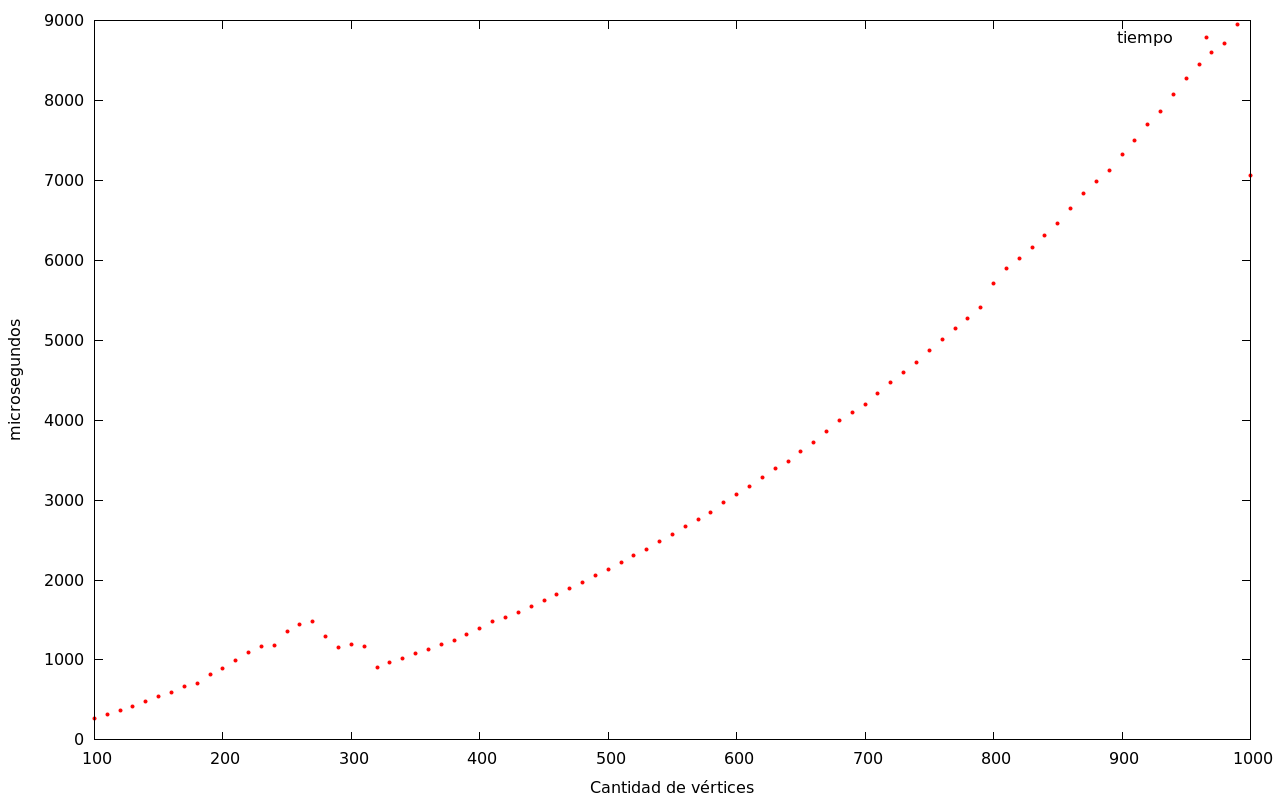
\includegraphics[scale=0.35]{imagenes/grafico-greedy-c.png}
  \end{center}
\end{figure}

\vspace{0.5cm}


\newpage
\subsubsection{Test 4 - algoritmo goloso, con aleatorización en aristas y conjuntos}

(ver \verb|info.2.k.dat|) \medskip

En este test, tenemos $n$ nodos, con $n$ inicializado en 100, incrementándose de a 10 hasta alcanzar 1000, $m$ inicializado en 500, incremendtándose de a 50 hasta alcanzar 5000 (vale 5 veces $n$) y $k$ vale $\frac{n}{20}$.

Para cada instancia se toma el \textbf{valor mínimo} mediado en microsegundos luego de \textbf{10 corridas}.

Dada una combinación de $m$, $n$ y $k$, se generaron 5 instancias aleatorias con dicha combinación y se consideró el promedio entre ellas.

\vspace*{0.5cm}

\begin{figure}[h]
  \begin{center}
    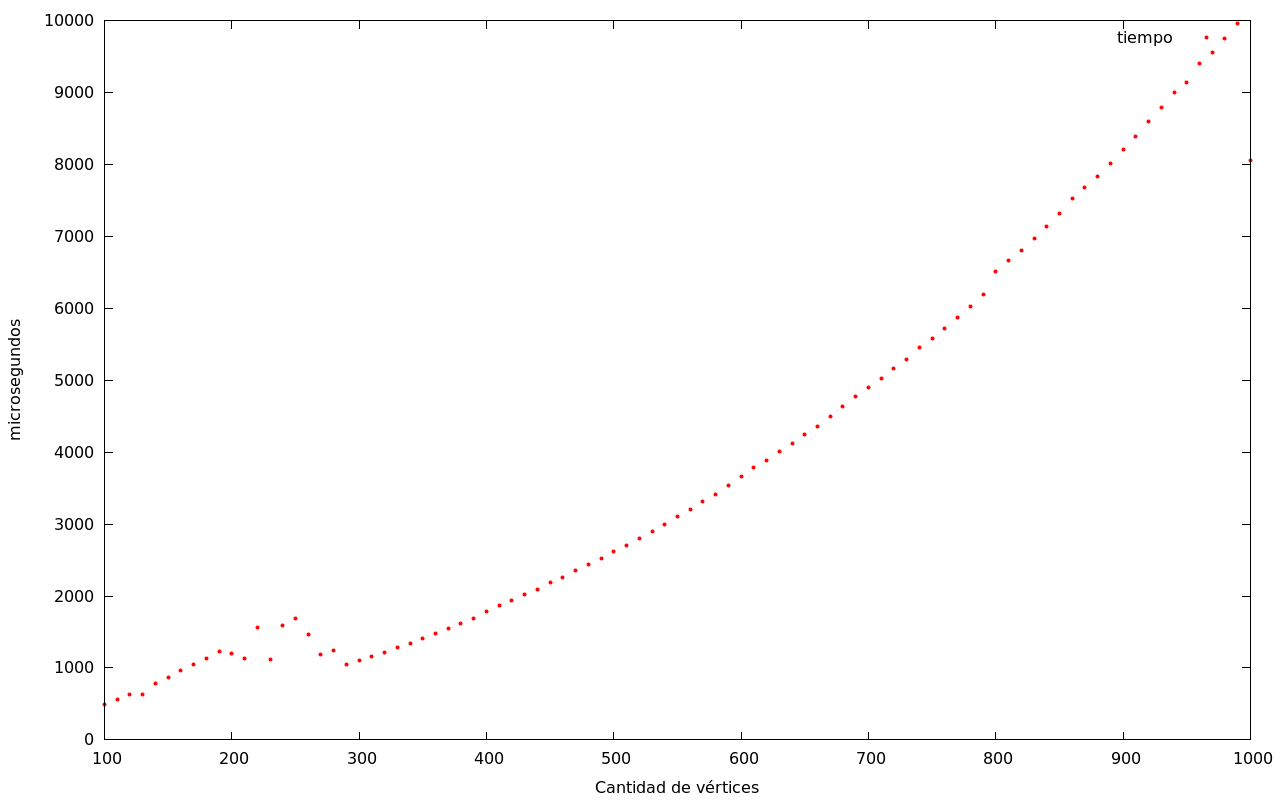
\includegraphics[scale=0.35]{imagenes/grafico-greedy.png}
  \end{center}
\end{figure}

\vspace{0.5cm}


